\section{Demonstration}
\begin{frame}{Simulatoren}
\begin{columns}
\begin{column}{0.6\textwidth}
Implementationen
\begin{itemize}
\item Dimensioner fra OpenStreetMap
\item SUMO: Mikrosimulator
\item Benytter "car-following-model"
\item Standardkørsel: Kører efter hastighedsgrænsen når muligt
\item Interfaced med TraCI
\item \tech skrevet i Python
\end{itemize}
\end{column}

\begin{column}{0.5\textwidth}
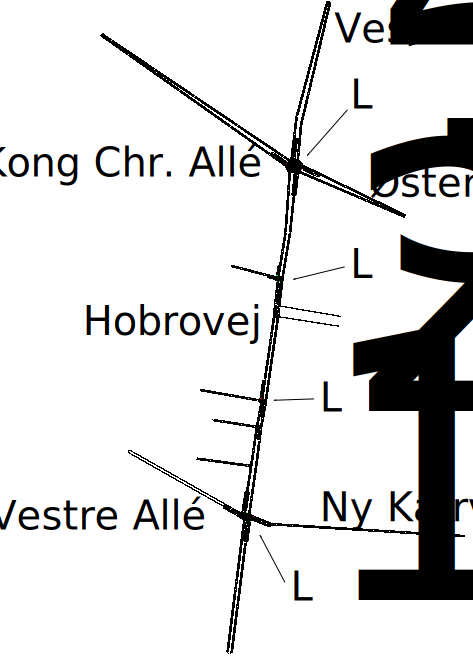
\includegraphics[width=1\textwidth]{../images/HobrovejNy.png}
\end{column}
\end{columns}
\end{frame}

\begin{frame}{Demonstration}
1. Alle kører efter simulatorens standardkørsel
\vspace{4mm}

2. Alle kører med \tech
\begin{itemize}
\item Viser virkningen bedst
\end{itemize}
\end{frame}
